\documentclass{standalone}

\usepackage[OT1]{fontenc}
\renewcommand*\familydefault{\sfdefault}
\usepackage{helvet,sfmath}
\usepackage{siunitx}

\usepackage{tikz}
\usetikzlibrary{arrows,calc,patterns}
% \usetikzlibrary{intersections, calc, arrows.meta}
\usepackage{tikz,tkz-euclide}

\begin{document}
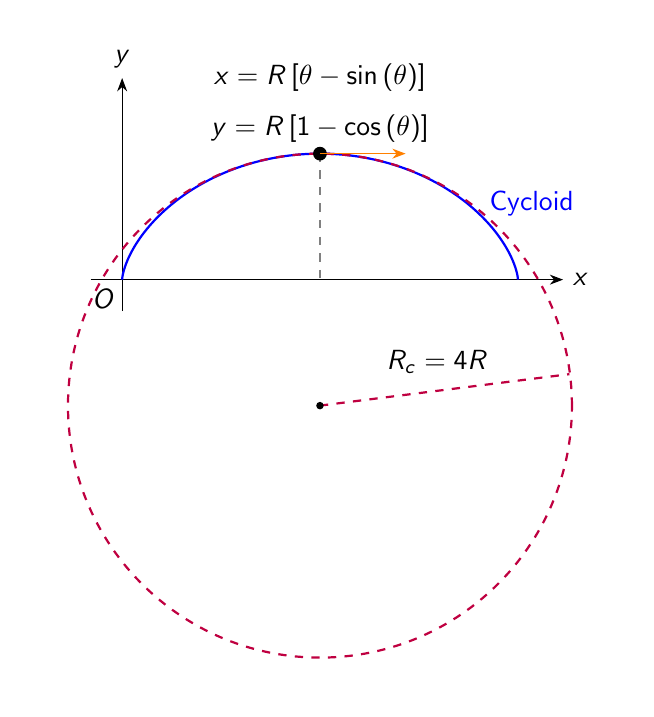
\begin{tikzpicture}[scale=0.8, >=Stealth]

    %% Background
    \draw[draw=none] (-1.5,-6.5) rectangle (8,4);

  % Trục tọa độ
  \draw[->] (-0.5, 0) -- (7, 0) node[right] {$x$};
  \draw[->] (0, -0.5) -- (0, 3.2) node[above] {$y$};
  \draw (-0.3,-0.3) node{\(O\)};

  % Đường cycloid
  \draw[thick, domain=0:6.28, samples=1000, variable=\t, smooth, blue]    plot ({(\t - sin(57.3*\t))}, {(1 - cos(57.3*\t)});

  % Nhãn quỹ đạo
  \node[blue] at (6.5,1.2) {Cycloid};

  % Tọa độ điểm cao nhất (t = 0)
  \coordinate (O) at (0,0);
  \coordinate (Top) at (3.14,2);

  % Vẽ bán kính cong tại đỉnh
  \draw[dashed, gray] (Top) -- ++(0,-2);
  \draw[purple, thick, dashed] (3.14,-2) circle (4);

  % Ghi chú bán kính cong
    \draw[purple, thick, dashed] (3.14,-2) to (7.1,-1.5);
    \draw[fill=black] (3.14,-2) circle (0.05);
    \draw (5,-1.3) node{\(R_c = 4 R\)};

  % Ghi chú điểm cao nhất
  \draw[fill=black] (3.14,2) circle (0.1);
  \draw[->, orange] (3.14,2) to (4.5,2);
  \draw 
  (3.14,3.2) node{\(x = R \left[ \theta - \sin \left( \theta \right) \right]\)}
  (3.14,2.4) node{\(y = R \left[ 1 - \cos \left( \theta \right) \right]\)}
  ;

\end{tikzpicture}

\end{document}
